\switchcolumn[1]*
\codeblock{basics/mc_fishers}
\codeblock{basics/mc_fisher_product}
\switchcolumn[0]

In Section ??
we have demonstrated that a neural network almost always models a likelihood for the labels given the inputs using parameters.
This perspective provides a new way to compare two models $f_1 \coloneq f(\bullet, \vtheta_1), f_2 \coloneq f(\bullet, \vtheta_{2})$ where $\vtheta_2 = \vtheta_1 + \Delta \vtheta$.
Instead of assessing their dissimilarity by their parameters' dissimilarity, e.g.\,using the Euclidean distance measure $d^2(f_1, f_2) = \left\lVert \vtheta_2 - \vtheta_1 \right\rVert_2^2 = \left\lVert \Delta \vtheta \right\rVert_2^2$, we could instead use the KL-divergence of the probability densities represented by the two networks, $d^2(f_1, f_2) = \mathrm{KL}(p(\rvx, \rvy \mid \vtheta_1) \mid\mid p(\rvx, \rvy \mid \vtheta_2))$.
% $\mathrm{KL}(r(\rvy \mid f(\vx, \vtheta_1)) \mid\mid r(\rvy \mid f(\vx, \vtheta_2)))$.
As $p(\rvx, \rvy \mid \vtheta) = p(\rvy \mid \rvx, \vtheta)p_{\sD}(\rvx)$, one can show that
\begin{align*}
    & \mathrm{KL}(p(\rvx, \rvy \mid \vtheta_1) \mid\mid p(\rvx, \rvy \mid \vtheta_2))                               \\
  = & \E_{p_{\sD}(\rvx)} [\mathrm{KL}(p(\rvy \mid \rvx, \vtheta_1) \mid\mid p(\rvy \mid \rvx, \vtheta_2))].
\end{align*}
For general pairs $(\vtheta_1, \vtheta_2)$, the KL divergence is not a valid distance measure though, e.g.\,it is not symmetric w.r.t.\,its arguments.
However, for small $\Delta \vtheta$, the KL divergence can be locally approximated by a quadratic Taylor series.
Assuming flattened parameter vectors, the Hessian showing up in this approximation is the Fisher information matrix and it implies a proper metric inside a small neighbourhood,
\begin{align*}
  \mathrm{KL}(p(\rvx, \rvy \mid \vtheta) \mid\mid p(\rvx, \rvy \mid \vtheta + \Delta \vtheta))
  \\
  = \frac{1}{2} {\Delta \vtheta}^{\top} \mF(\vtheta) \Delta \vtheta + \gO( \Vert\Delta \vtheta\Vert^3)\,.
\end{align*}
with the Fisher information matrix
\begin{align*}
  \mF(\vtheta) = \E_{p(\rvx, \rvy \mid \vtheta)} [-\hess_{\vtheta} \log p(\rvx, \rvy \mid \vtheta)]\,.
\end{align*}
Let's rewrite this expression in terms of the likelihood $p(\rvy \mid \vx, \vtheta)$, and its reparameterized likelihood $r(\rvy \mid f(\rvx, \vtheta))$,
\begin{align*}
  \mF(\vtheta)
   & =
  \E_{p_{\sD}(\rvx)}\E_{p(\rvy \mid \rvx, \vtheta)} [-\hess_{\vtheta} \log p(\rvy \mid \rvx, \vtheta)]\,.
  \\
   & =
  \E_{p_{\sD}(\rvx)}\E_{r(\rvy \mid f(\rvx, \vtheta))} [-\hess_{\vtheta} \log r(\rvy \mid f(\rvx, \vtheta))]\,.
\end{align*}
\paragraph{Type-II Fisher:} In practise, we must replace the true marginal distribution over the inputs with its empirical distribution $p_{\sD}(\rvx) = \frac{1}{N}\sum_n \delta(\rvx - \vx_n)$. We will call the resulting matrix the type-II Fisher information matrix (because it is defined via second-order derivatives of the likelihood) and use the abbreviation $\vf_n \coloneq f(\rvx = \vx_n, \vtheta)$,
\begin{align*}
  \mF^{\text{II}}(\vtheta)
   & =
  \E_{p_{\sD}(\rvx)}\E_{r(\rvy \mid f(\rvx, \vtheta))} [-\hess_{\vtheta} \log r(\rvy \mid f(\rvx, \vtheta))]\,.
  \\
   & =
  \frac{1}{N} \sum_n
  \E_{r(\rvy \mid \vf_n)} [-\hess_{\vtheta} \log r(\rvy \mid \vf_n)]\,.
\end{align*}
We can apply the chain rule to the Hessian of the log-likelihood and use the fact that $\E_{r(\rvy \mid f(\rvx, \vtheta))}[\nabla_{f(\rvx, \vtheta)} \log r(\rvy \mid f(\rvx, \vtheta))] = \vzero$ to simplify the type-II Fisher into
\begin{align*}
  \mF^{\text{II}}(\vtheta) & = \frac{1}{N} \sum_n \E_{r(\rvy \mid \vf_n)} [
  \begin{aligned}[t]
     & {\jac_{\vtheta} \vf_n}^{\top}                          \\
     & \left( -\hess_{\vf_n} \log r(\rvy \mid \vf_n)  \right) \\
     & \jac_{\vtheta} \vf_n ]\,
  \end{aligned}
  \shortintertext{and, as Jacobians do not depend on $\rvy$,}
                           & = \frac{1}{N} \sum_n
  \begin{aligned}[t]
     & {\jac_{\vtheta} \vf_n}^{\top} \\
     & \left(
    \E_{r(\rvy \mid \vf_n)} [
        -\hess_{\vf_n} \log r(\rvy \mid \vf_n)
      ]
    \right)                          \\
     & \jac_{\vtheta} \vf_n \,.
  \end{aligned}
\end{align*}

\paragraph{Type-I Fisher:} There is another way to rewrite the Fisher information matrix in terms of first-order derivatives of the log-likelihood.
We will call this the type-I Fisher information matrix.
To derive it, we use the property that the negative log-likelihood's Hessian equals its gradient covariance in expectation,
\begin{align*}
    & \E_{p(\rvx, \rvy \mid \vtheta)}
  \left[
    -\hess_{\vtheta} \log p(\rvx, \rvy \mid \vtheta)
    \right]
  \\
  = & \E_{p(\rvx, \rvy \mid \vtheta)} [
    \begin{aligned}[t]
       & (-\nabla_{\vtheta} \log p(\rvx, \rvy \mid \vtheta)) \\
       & (-\nabla_{\vtheta} \log p(\rvx, \rvy\mid  \vtheta))^{\top}]
    \end{aligned}
\end{align*}
Hence, we can write the Fisher as
\begin{align*}
  &\mF(\vtheta)
  \\
               & = \E_{p(\rvx, \rvy \mid \vtheta)} [
    \begin{aligned}[t]
       & (-\nabla_{\vtheta} \log p(\rvx, \rvy \mid \vtheta))        \\
       & (-\nabla_{\vtheta} \log p(\rvx, \rvy \mid \vtheta))^{\top}]
    \end{aligned}
  \\
               & = \E_{p_{\sD}(\rvx)}\E_{p(\rvy \mid \rvx, \vtheta))} [
    \begin{aligned}[t]
       & (-\nabla_{\vtheta} \log p(\rvy \mid \rvx, \vtheta))        \\
       & (-\nabla_{\vtheta} \log p(\rvy \mid \rvx, \vtheta))^{\top}]
    \end{aligned}
  \\
               & = \E_{p_{\sD}(\rvx)}\E_{r(\rvy \mid f(\rvx, \vtheta))} [
    \begin{aligned}[t]
       & (-\nabla_{\vtheta} \log r(\rvy \mid f(\rvx, \vtheta)))        \\
       & (-\nabla_{\vtheta} \log r(\rvy \mid f(\rvx, \vtheta)))^{\top}]
    \end{aligned}
\end{align*}
Let's apply the chain rule for the gradient, substitute the empirical distribution for $p_{\sD}(\rvx)$ and simplify the notation using $\vf_n \coloneqq f(\rvx = \vx_n, \vtheta)$,
\begin{align*}
  & \mF^{\text{I}}(\vtheta)
 \\
  & =
 \frac{1}{N} \sum_n
 \E_{r(\rvy \mid \vf_n)}
 [\begin{aligned}[t]
   & (-\nabla_{\vtheta} \log r(\rvy \mid \vf_n)) \\
   & (-\nabla_{\vtheta} \log r(\rvy \mid \vf_n))^{\top}]
 \end{aligned}
 \\
  & =
 \frac{1}{N} \sum_n
 \E_{r(\rvy \mid \vf_n)}
 [\begin{aligned}[t]
   & (\jac_{\vtheta}\vf_n)^{\top} \\
   & (-\nabla_{\vf_n} \log r(\rvy \mid \vf_n)) \\
   & (-\nabla_{\vf_n} \log r(\rvy \mid \vf_n))^{\top} \\
   & \jac_{\vtheta}\vf_n]
 \end{aligned}
 \\
 \shortintertext{and, as Jacobians do not depend on $\rvy$,}
  & =
 \frac{1}{N} \sum_n
 \begin{aligned}[t]
   & (\jac_{\vtheta}\vf_n)^{\top} \\
   & \E_{r(\rvy \mid \vf_n)}
   [(-\nabla_{\vf_n} \log r(\rvy \mid \vf_n)) \\
   & \phantom{\E_{r(\rvy \mid \vf_n)}[}(-\nabla_{\vf_n} \log r(\rvy \mid \vf_n))^{\top}] \\
   & \jac_{\vtheta}\vf_n \,.
 \end{aligned}
\end{align*}

\paragraph{Monte-Carlo approximation of the Fisher:} In practise, we need to replace the expectation over $r(\rvy \mid \vf_n)$ with an estimator, e.g.\,a Monte-Carlo approximation with $M$ sampled labels $\tilde{\vy}_{n,1}, \dots, \tilde{\vy}_{n, M} \stackrel{\text{i.i.d}}{\sim} r(\rvy \mid \vf_n)$ for the prediction of datum $n$.

\begin{definition}[Monte-Carlo-approximated Type-I Fisher (\Cref{mc_fishers})]\label{def:mc_fisher}%
  The Monte-Carlo-approximated type-I Fisher matrix of the likelihood $\log r(\rvy \mid f(\vx_n, \vtheta))$,
  $\tilde{\mF}^{\text{I}}(\vtheta) \in \sR^{D \times D}$ is defined as
  \begin{align*}
    & \tilde{\mF}^{\text{I}}(\vtheta) \\
	& = \frac{1}{NM} \sum_{n,m}
	\begin{aligned}[t]
	   & (-\nabla_{\vtheta} \log r(\rvy = \tilde{\vy}_{n,m} \mid \vf_n))        \\
	   & (-\nabla_{\vtheta} \log r(\rvy = \tilde{\vy}_{n,m} \mid \vf_n))^{\top} \\
	\end{aligned} \\
    & = \frac{1}{NM} \sum_{n,m}
    \begin{aligned}[t]
       & \left(\jac_{\vtheta}\vf_n\right)^{\top}                              \\
       & (-\nabla_{\vf_n} \log r(\rvy = \tilde{\vy}_{n,m} \mid \vf_n))        \\
       & (-\nabla_{\vf_n} \log r(\rvy = \tilde{\vy}_{n,m} \mid \vf_n))^{\top} \\
       & \jac_{\vtheta}\vf_n.
    \end{aligned}
  \end{align*}
\end{definition}

\switchcolumn[1]
\begin{figure}
  \centering
  \begin{minipage}[t]{0.495\linewidth}
    \centering
    $\cvec 1$ sample\vspace{1ex}
    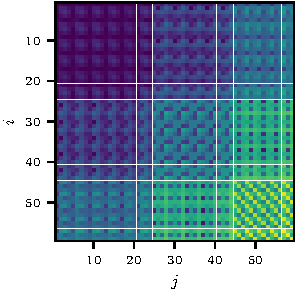
\includegraphics[width=0.8\linewidth]{../kfs/plots/synthetic_cvec_mcfisher_1.pdf}
  \end{minipage}
  \hfill
  \begin{minipage}[t]{0.495\linewidth}
    \centering
    $\rvec 1$ sample\vspace{1ex}
    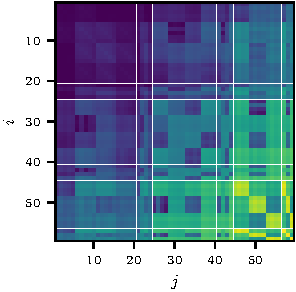
\includegraphics[width=0.8\linewidth]{../kfs/plots/synthetic_rvec_mcfisher_1.pdf}
  \end{minipage}
  \\
  \begin{minipage}[t]{0.495\linewidth}
    \centering
    $\cvec 100$ samples\vspace{1ex}
    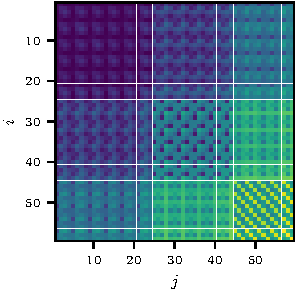
\includegraphics[width=0.8\linewidth]{../kfs/plots/synthetic_cvec_mcfisher_100.pdf}
  \end{minipage}
  \hfill
  \begin{minipage}[t]{0.495\linewidth}
    \centering
    $\rvec 100$ samples\vspace{1ex}
    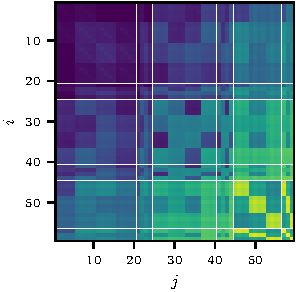
\includegraphics[width=0.8\linewidth]{../kfs/plots/synthetic_rvec_mcfisher_100.pdf}
  \end{minipage}
  \begin{minipage}[t]{0.495\linewidth}
    \centering
    $\cvec$ exact\vspace{1ex}
    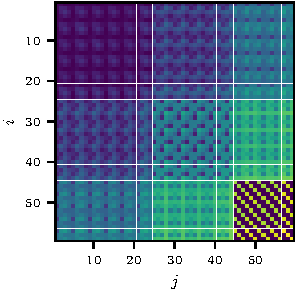
\includegraphics[width=0.8\linewidth]{../kfs/plots/synthetic_cvec_ggn.pdf}
  \end{minipage}
  \hfill
  \begin{minipage}[t]{0.495\linewidth}
    \centering
    $\rvec$ exact\vspace{1ex}
    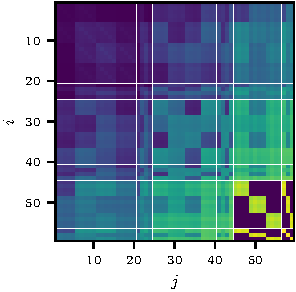
\includegraphics[width=0.8\linewidth]{../kfs/plots/synthetic_rvec_ggn.pdf}
  \end{minipage}
  \begin{minipage}[t]{0.495\linewidth}
    \centering
    $\cvec$ empirical\vspace{1ex}
    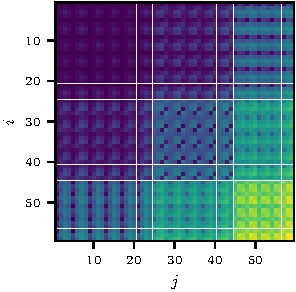
\includegraphics[width=0.8\linewidth]{../kfs/plots/synthetic_cvec_empfisher.pdf}
  \end{minipage}
  \hfill
  \begin{minipage}[t]{0.495\linewidth}
    \centering
    $\rvec$ empirical\vspace{1ex}
    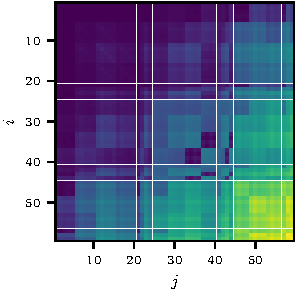
\includegraphics[width=0.8\linewidth]{../kfs/plots/synthetic_rvec_empfisher.pdf}
  \end{minipage}
  \caption{Visualization of the Monte-Carlo-approximated Fisher using different flattening schemes and number of MC samples.
    The Fisher blocks are visually highlighted with white lines.
    Left column uses $\cvec$-flattening, right column uses $\rvec$-flattening.
    The penultimate row uses the exact Fisher. The last row shows the empirical Fisher, highlighting its difference to the previous curvature estimates.
    The Fishers were evaluated on synthetic data ($N=100$) using an MLP with three fully-connected layers and ReLU activations (5-4-4-3, our notation considers applying the weight matrix and adding the bias as two layers, hence $L=6$) and square loss.
  }
\end{figure}

\begin{figure}
  \centering
  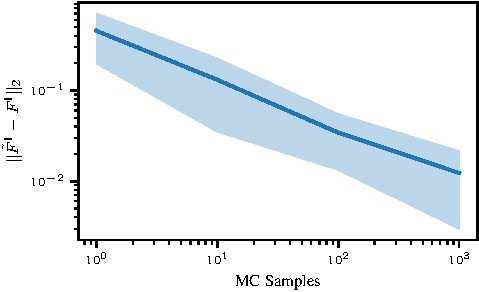
\includegraphics[width=\linewidth]{../kfs/plots/synthetic_rvec_diff_spec_norm.pdf}
  \caption{Visualization of the difference spectral norm between the Monte-Carlo-approximated and exact type-I Fishers as a function of the number of MC samples.
    The Fishers were evaluated on synthetic data ($N=100$) using an MLP with three fully-connected layers and ReLU activations (5-4-4-3, our notation considers applying the weight matrix and adding the bias as two layers, hence $L=6$) and square loss.
  }
\end{figure}

\switchcolumn[0]

Let's denote the $m$-th negative would-be gradient for sample $n$ by $\tilde{\vg}_{n,m} \coloneq -\nabla_{\vf_n} \log r(\rvy = \tilde{\vy}_{n,m} \mid \vf_n)$
We can then form the matrix
\begin{align*}
  \tilde{\mS}_n
  \coloneq
  \frac{1}{\sqrt{M}}
  \begin{pmatrix}
    \tilde{\vg}_{n,1} & \cdots & \tilde{\vg}_{n,M}
  \end{pmatrix}
  \in \sR^{C \times M}
\end{align*}
for each $n$, and express the MC-approximated Fisher as
\begin{align*}
  \tilde{\mF}^{\text{I}}(\vtheta)
   & =
  \frac{1}{N} \sum_{n,m}
  (\jac_{\vtheta}\vf_n)^{\top}
  \tilde{\mS}_n
  \tilde{\mS}_n^{\top}
  \jac_{\vtheta}\vf_n
  \\
   & =
  \frac{1}{N} \sum_n
  \tilde{\mV}_n
  \tilde{\mV}_n^{\top}
\end{align*}
where $\tilde{\mV}_n \in \sR^{D \times M}$.
Did you notice what we just did here?
By stacking the negative would-be gradients into columns of a matrix, we were able to express the Fisher as the self-outer product of a matrix $\tilde{\mV}_n$.
This notation looks very similar to the GGN's self-outer product notation.
We can think of $\tilde{\mV}_n \in \sR^{D \times M}$ as a randomization of $\mV_n \in \sR^{D \times C}$ which can be much smaller (depending on the choice of $M$) and therefore cheaper to compute.

\paragraph{Reduction factor of the Fisher versus empirical risk:}
In the above derivation we arrived at an expression of the Fisher which uses a reduction factor $R = \frac{1}{N}$.
However, other reduction factors are equally common, e.g.\,when predicting a sequence of $T$ tokens, the reduction factor is $R = \frac{1}{NT}$.
In other words, the Fisher is tied to a statistical manifold over probability distributions, and depending on our choice of distribution, we obtain different normalizations.
This is a subtlety that we will usually ignore in practise, simply by using the reduction factor from our empirical risk (which consequently implies the statistical manifold on which we are considering the Fisher).


\begin{example}[Gradients of MSELoss]
  Consider the square loss from \Cref{ex:square_loss} and its probabilistic interpretation from \Cref{ex:square_loss_probabilistic}
  For some label $\vy$, the gradient is given by
  \begin{align*}
    \nabla_{\vf} c(\vf, \vy)
     & =
    - \nabla_{\vf} \log r(\rvy =\vy \mid \vf)
    \\
     & =
    \vf - \vy\,.
  \end{align*}
\end{example}

\begin{example}[Gradients of CrossEntropyLoss]
  Consider the softmax cross-entropy loss from \Cref{ex:cross_entropy_loss} and its probabilistic interpretation from \Cref{ex:cross_entropy_loss_probabilistic}. For some label $y$, the gradient is given by
  \begin{align*}
    \nabla_{\vf} c(\vf, y)
     & =
    - \nabla_{\vf} \log r(\ry = y \mid \vf)
    \\
     & =
    p(\vf) - \mathrm{onehot}(y)\,.
  \end{align*}
\end{example}

%%% Local Variables:
%%% mode: latex
%%% TeX-master: "../main"
%%% End:
